\section{Entscheidungsprozesse}

\begin{frame}[c]{Fehlerquellen in Entscheidungsprozessen}
    \centering
    % Folie langsam aufbauen, ist sonst zu viel information auf einmal
    % Konkretes Beispiel!!
    % ideen: Kaufen eines Produktes im Supermarkt
    % idee: Terminoptimierung - Freizeitoption A oder B, fokus auf Gruppendynamik
    % \only<1>{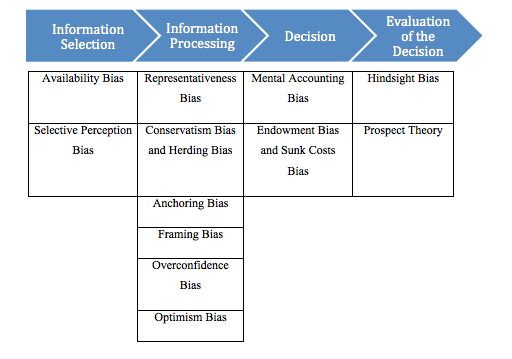
\includegraphics[width=\textwidth, clip=true, trim= 0mm 102mm 0mm 0mm]{DecisionMakingProcedure}}
    \only<1->{
\includegraphics[width=\textwidth]{DecisionMakingProcedure0}\vfill}
%     \only<2>{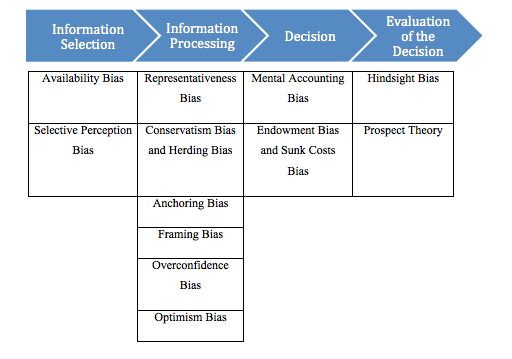
\includegraphics[width=\textwidth]{DecisionMakingProcedure}}
\end{frame}

\begin{frame}[c]{Entscheidungsprozesse - Beispiel}
    \Large
    Situation: Man möchte ein neues Handy kaufen. \\
\end{frame}


\begin{frame}[c]{Kaufen eines neuen Handys}
    
\includegraphics[width=\textwidth]{Sammeln_Informationen0} \\
    Hier müssen wir vor allem aufpassen bezüglich:
    \begin{itemize}[<+(1)->]
        \item Verzerrungen der Verfügbarkeit
            % Jemand hat erst am Tag zuvor ein Handy empfohlen vs Länger zuvor
        \item Selektiver Wahrnehmung
            % Die Tendenz, genau das zu sehen das man sehen möchte
        \item Bestätigungsvoreingenommenheit
            % Man sucht, interpretiert und beschäftigt sich hauptsächlich mit bestätigenden informationen
        \item Frequenzillusion
            % Frequenzen werden üblicherweise unverständlich dargestellt
    \end{itemize}
    (von Informationen)
\end{frame}


\begin{frame}[c]{Kaufen eines neuen Handys}
    
\includegraphics[width=\textwidth]{Informations_Verarbeitung0} \\
    Hier müssen wir vor allem aufpassen bezüglich:
    \begin{itemize}[<+(1)->]
        \item Repräsentativität
            % Marken stehen für bestimmte dinge
        \item Ankereffekt/Rahmungseffekt
            % Sobald wir einen Wert 'Ankern' werden wir nicht mehr sehr viel davon abweichen
            % Wie etwas Präsentiert wird beinflusst unsere Wahrnehmung davon
        \item Optimismus/Übersteigertes Selbstvertrauen
            % die welt ist nicht so gut wie man sie manchmal gerne hätte
        \item Gruppenzwang
            % eingehen auf Empfehlungen anderer, unabhängig davon ob es für einen selbst passt
        \item Konservativität
            % Nicht direktes einbeziehen neuer Informationen
    \end{itemize}
\end{frame}


\begin{frame}[c]{Kaufen eines neuen Handys}
    
\includegraphics[width=\textwidth]{Entscheidung0} \\
    Hier müssen wir vor allem aufpassen bezüglich:
    \begin{itemize}[<+(1)->]
        \item Schubladendenken (Mental Accounting Bias)
            % Alles ist entweder Gut oder Schlecht
        \item Besitztum (Endowment Bias)
            % sobald man etwas einmal besitzt möchte man es nicht wieder hergeben
        \item Täuschung der investierten Kosten
            % 'sunk cost bias', man möchte dass sich etwas auch lohnt
        \item Wählen des Üblichen
            % 'Default effect', man wählt das übliche auch bei neuen möglichkeiten
        \item Gesetz des Instruments
            % übermäßiges verwenden eines einzelnen Werkzeuges
    \end{itemize}
\end{frame}


\begin{frame}[c]{Kaufen eines neuen Handys}
    
\includegraphics[width=\textwidth]{Bewertung0} \\
    Hier müssen wir vor allem aufpassen bezüglich:
    \begin{itemize}[<+(1)->]
        \item Rückschaufehler (Hindsight)
            % Im nachhinein scheinen dinge offensichtlich
        \item Eigennützigkeit (Self-Serving bias)
            % Interpretieren von neutraler Information zum eigenen Nutzen
        \item Gültigkeitsillusion (Illusion of validity)
            % Glaube dass entscheidungen bei wenig (zusammenhängender/konsistenter) Information richtig waren
        \item Fokussierung
            % Zu großer Fokus auf einen einzelnen Aspekt
        \item Nachträgliche Begründungstendenz
            % überzeugen eines selbst dass der Einkauf gut war
    \end{itemize}
\end{frame}




\begin{frame}[standout]
    ... und das ist nur ein kleiner Auszug.
\end{frame}

\begin{frame}[c]{List of cognitive Biases}
    \centering
    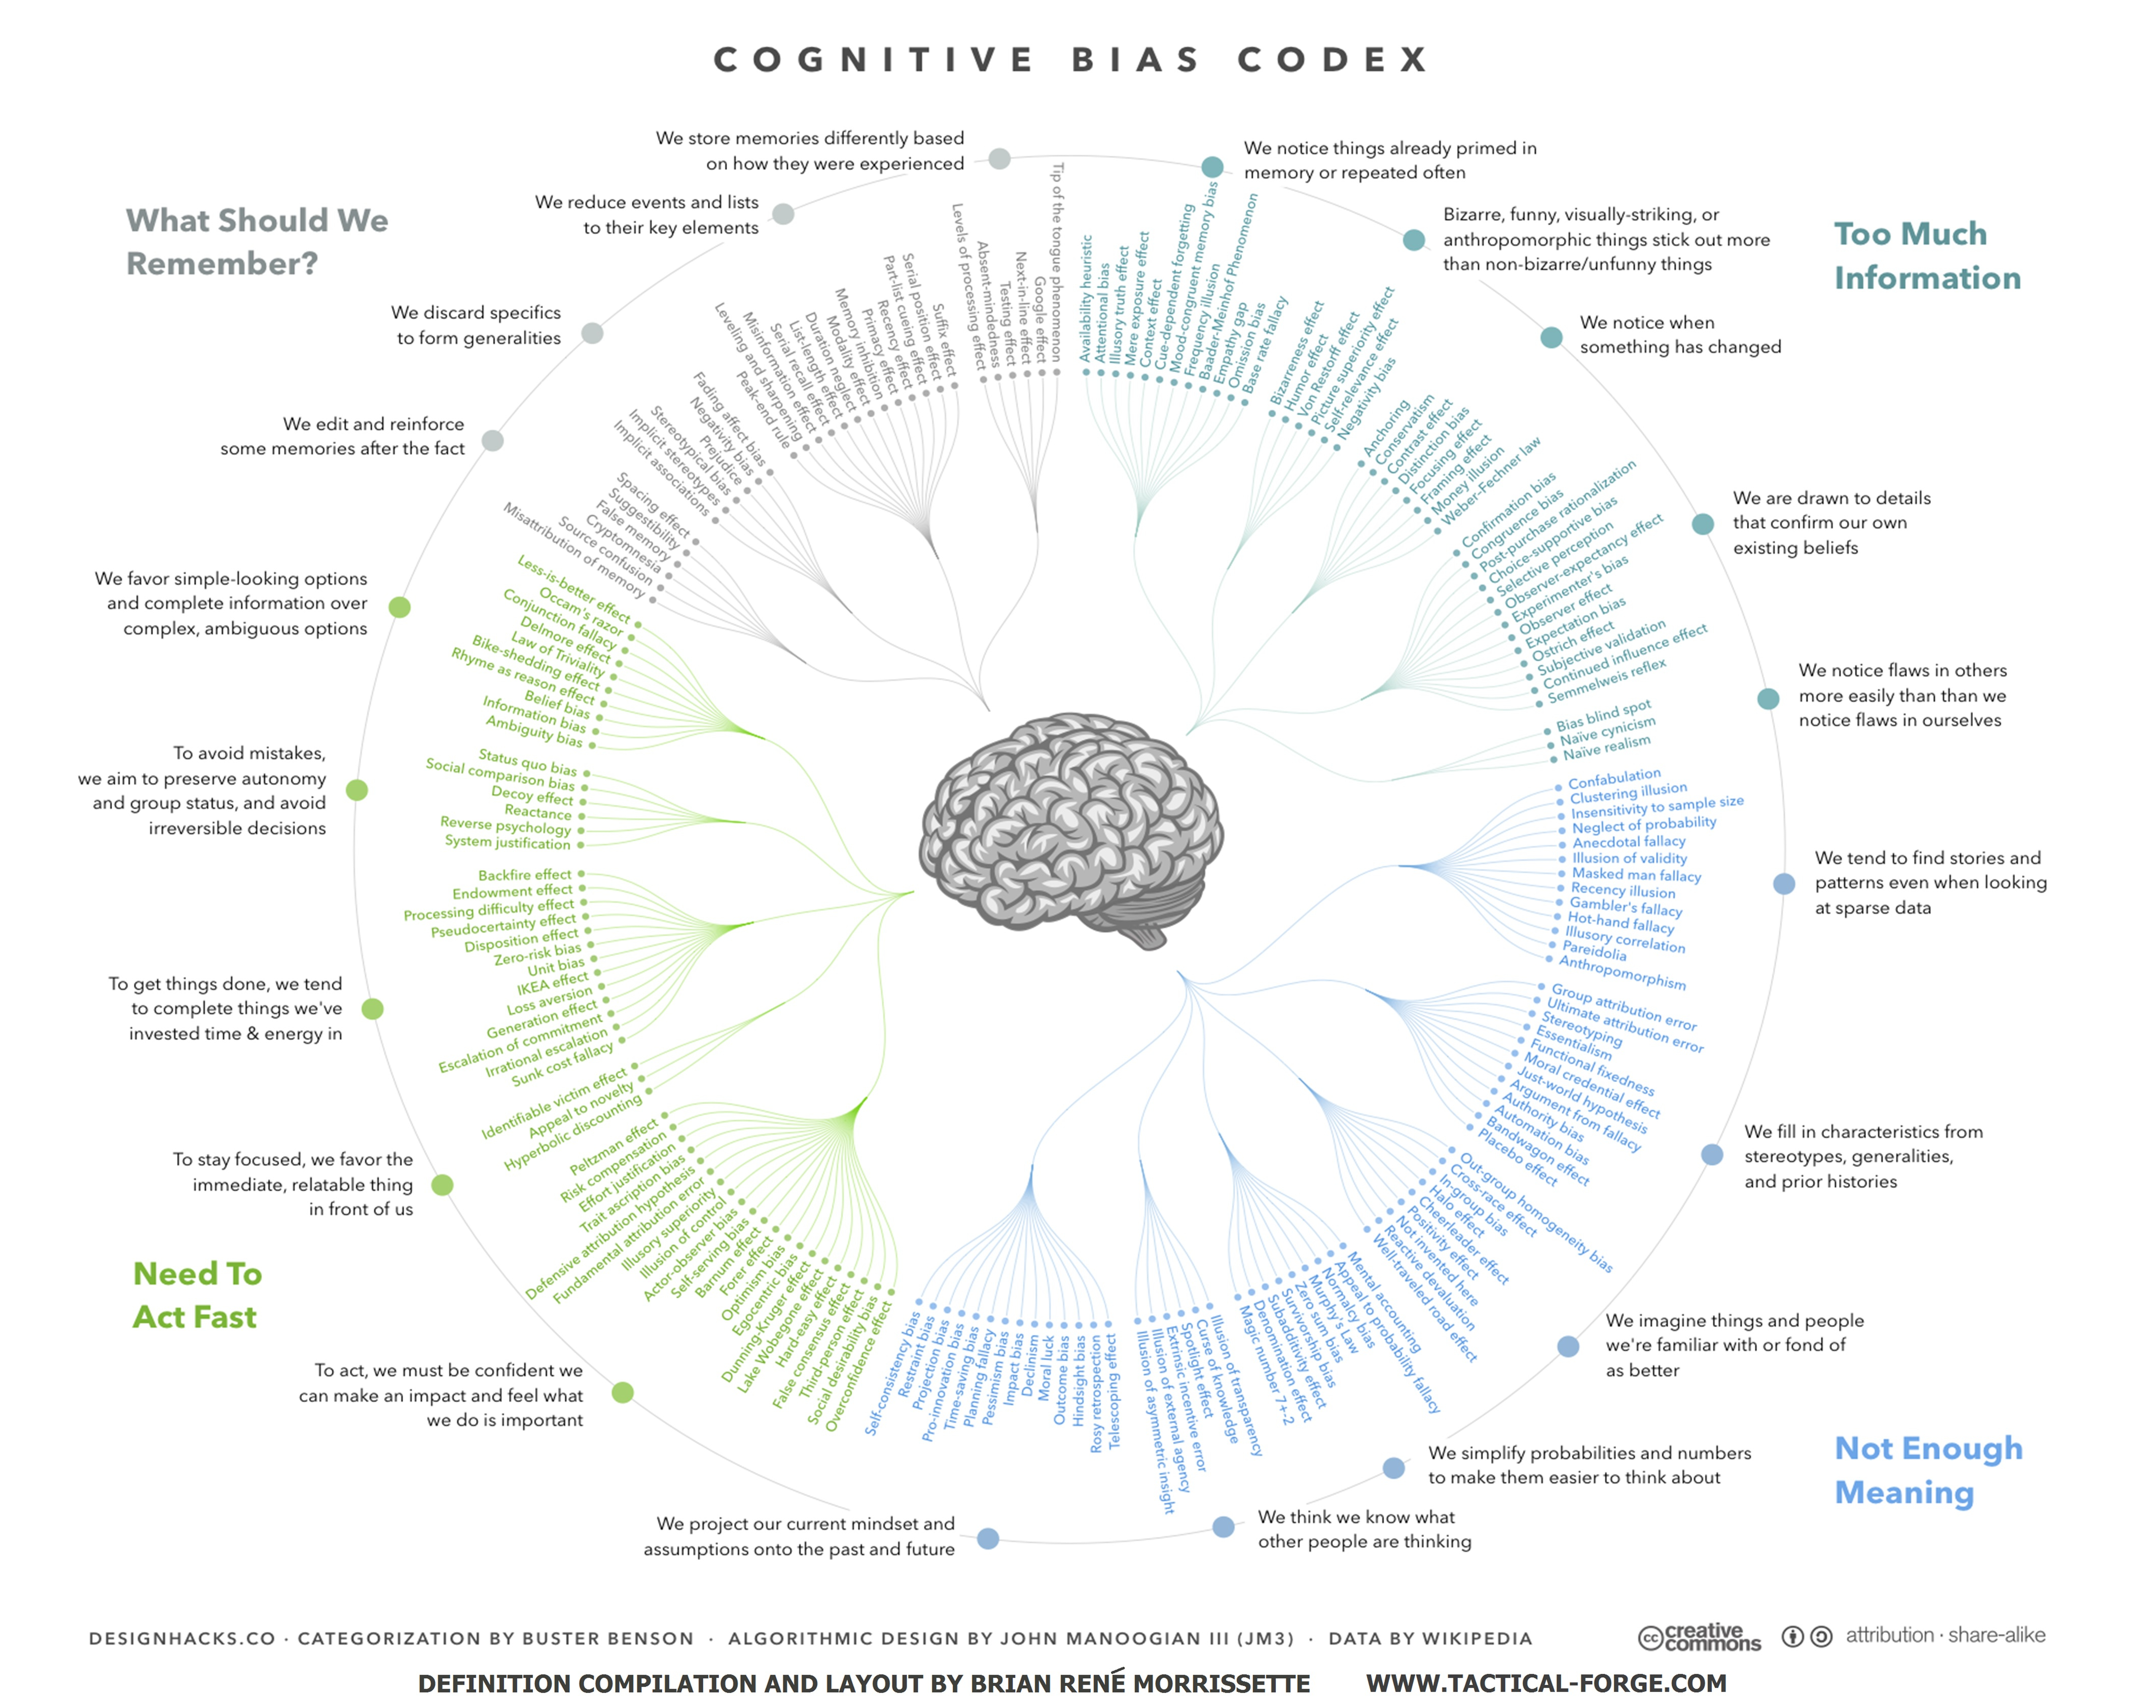
\includegraphics[width=\textwidth]{cogbias_0}
\end{frame}



\begin{frame}[c]{Wie funktioniert menschliches Denken?}
    \Large
    \pause
    % Das Gehirn arbeitet üblicherweise mit zwei verschiedenen Systemen
    \begin{itemize}
    \item System I - schnell, ungenau, einfach
    \newline
    \pause
    \item System II - langsam, ungenau, anstrengend
    \newline
    \pause
    \end{itemize}
    Was also tun?
\end{frame}



\begin{frame}[standout]
    Disclaimer: bias blind spot
\end{frame}



